% !TEX root =  ../../Krantz_style.tex

\label{sec:model} 
%We define here a hierarchically supervised LDA
%model. Although we will focus on document modeling in our description
%and experiments, this model applies equally well to other collections
%of discrete data with hierarchically constrained labels. 

This model (HSLDA) is designed to fit hierarchically, multiply-labeled, bag-of-word data.  We
call groups of bag-of-words data documents (unordered words in text documents, bag of visual feature representations of images, etc.).  Let $w_{n,d}
\in \Sigma$ be the $n$th observation in the $d$th document.  Let $\mathbf{w}_d
= \{w_{1,d},\ldots,w_{1,N_d}\}$ be the  set of $N_d$ observations in document
$d$.  Let there be $D$ such documents and let the size of the vocabulary be
$V=|\Sigma|$.  

Let the set of labels be $\mathcal{L}=\left\{
  l_{1},l_{2},\ldots,l_{\left|\mathcal{L}\right|}\right\} $.  A label in HSLDA corresponds to a node in the graphical model in Figure~\ref{fig:graphical_model}.  A label can either be observed or unobserved.  Documents can be multiply labeled, meaning that subsets of label nodes in the graphical model in Fig.~\ref{fig:graphical_model} can have observed values.  Each label
$l \in \mathcal{L}$, except the root, has a parent $\mathrm{pa}(l) \in \mathcal{L}$
also in the set of labels. 
 We will for exposition purposes assume that this label set has hard ``is-a''
 parent-child constraints (explained later), although this assumption can be
 relaxed at the cost of more computationally complex inference.  Such a label hierarchy forms a multiply rooted tree.   Confused readers may wish to consult Figure \ref{fig:diagnosis_tree} or Figure \ref{fig:product_tree} each of which is a  label-tree graphical model.  
 
 In a label forest a node may be observed (the label was ``applied'' and, for instance, was observed to have value 1), unobserved and unknown, or unobserved and constrained to be either -1 or 1 by the structure of the label space.   Without loss of generality we will consider a tree with a single root $r\in\mathcal{L}$.  Each document has a variable $y_{l,d} \in \{-1,1\}$ for every label which indicates whether the label applies to document $d$ or not.   In most cases $y_{l,d}$ will be unobserved, in some cases we will be able to fix its value because of  constraints on the label hierarchy, and in the relatively minor remainder its value will be observed.  In the applications we demonstrate, only positive labels are observed.   This may not be true of all applications; however, positive-only label imbalance is a common problem.  How we solve this problem will be discussed later.
 
The constraints imposed by an is-a label hierarchy are that if the $l$th label is applied to document $d$, i.e.,~$y_{l,d} = 1$, then all labels in the label hierarchy up to the root are also applied to document $d$, i.e.,~$y_{\mathrm{pa}(l),d} = 1, y_{\mathrm{pa}(\mathrm{pa}(l)),d} = 1, \ldots, y_{r,d}=1.$  Conversely, if a label $l'$ is marked as not applying to a document (i.e.~$y_{l',d}=-1$) then no descendant label of that label can take value 1.   We assume that at least one label is applied to every document.  This is illustrated in Figure~\ref{fig:graphical_model} where the root label is always applied but only some of the descendant labelings are observed as having been applied (diagonal hashing indicates that potentially some of the plated variables are observed).
%To reiterate, these is-a label hierarchy constraints can be relaxed.
%To capture this hierarchical structure we model the labeling of documents
%using a generative cascade of conditional probit regression models.

% generalize to arbitrary codes (not just ICD-9's
%
\begin{figure}[t]
%tbp] %  figure placement: here, top, bottom, or page
 \centering 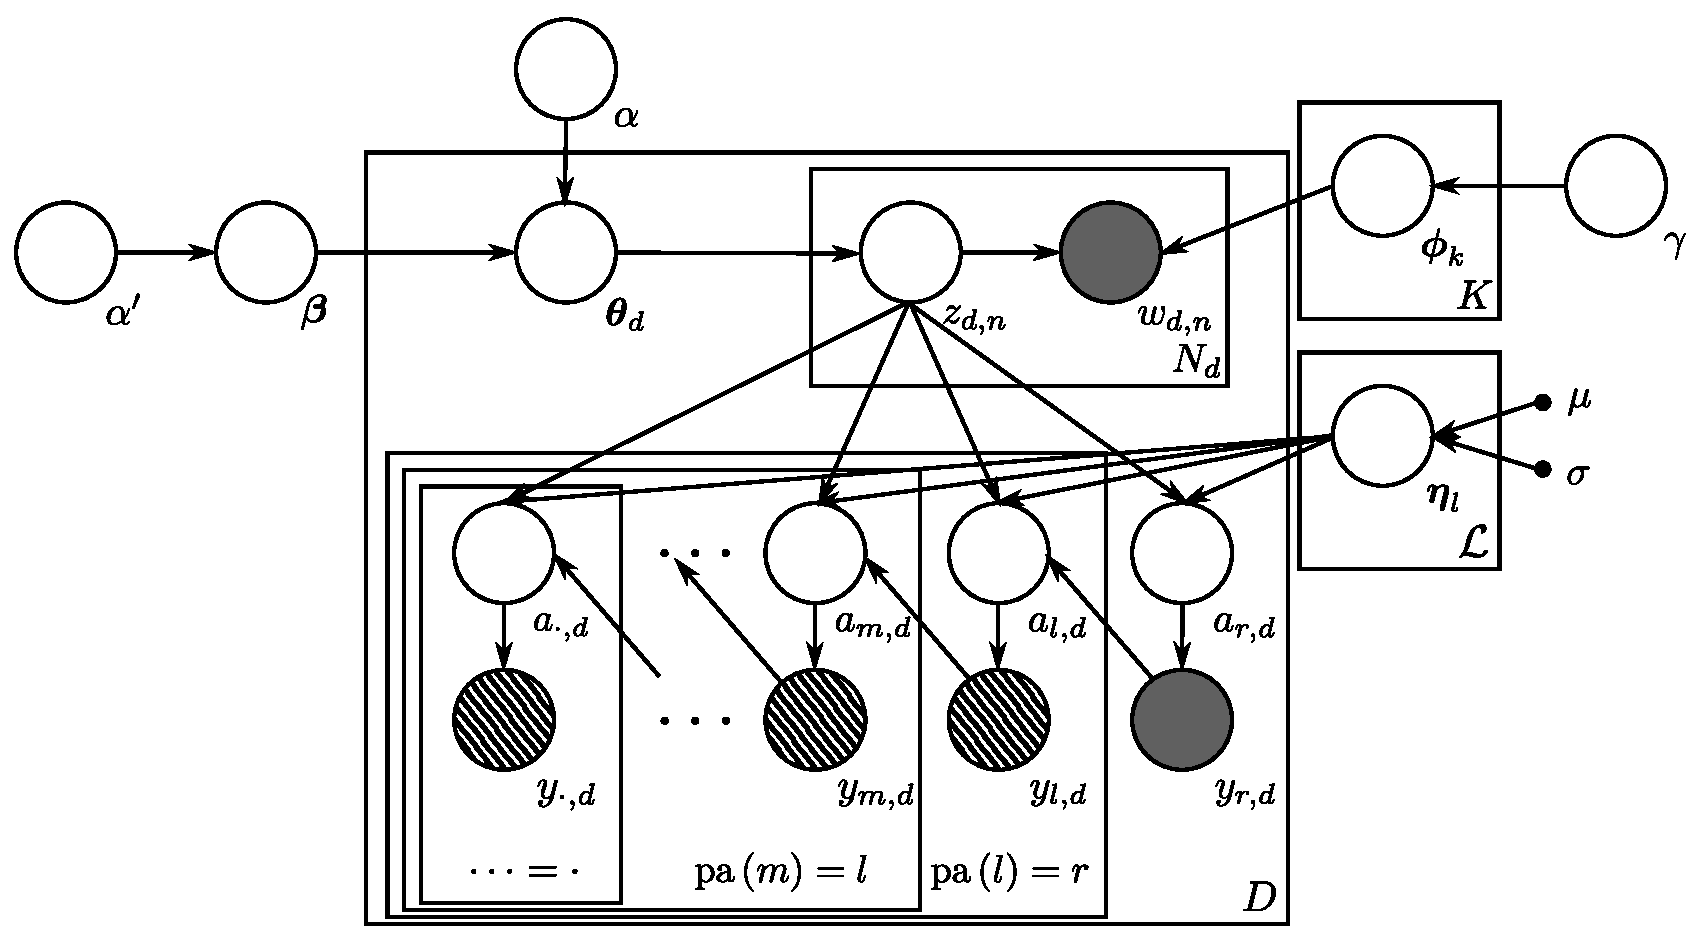
\includegraphics[scale=0.4]{Chapters/chapter1/Graphical_Model-final} \caption{Hierarchically supervised latent Dirichlet allocation (HSLDA) graphical model.}


\label{fig:graphical_model} 
\end{figure}

In HSLDA, the bag-of-word document data is modeled using LDA with
 full, hierarchical topic estimation (i.e. global topic proportions are also estimated).
%In HSLDA, documents are modeled using the LDA mixed-membership mixture model
%with global topic estimation. 
Label responses are modeled using a conditional
hierarchy of probit regressors and will be discussed next. The full HSLDA graphical model is given in
Figure~\ref{fig:graphical_model}.

 

\subsection{Generative Model}

In the following box  the HSLDA generative model  is given for the ``is-a hierarchy'' set of label constraints.   In the box and what follows in this chapter, $K$ is the number of LDA
``topics'' (distributions over the elements of $\Sigma$), $\boldsymbol\phi_k$
is a distribution over ``words,'' $\boldsymbol\theta_d$ is a document-specific
distribution over topics, $\boldsymbol\beta$ is a global distribution over
topics, Dir$_{K}(\cdot)$ is a $K$-dimensional Dirichlet distribution,
$\mathcal{N}_{K}(\cdot)$ is the $K$-dimensional Normal distribution,
$\mathbf{I}_{K}$ is the $K$ dimensional identity matrix,  $\mathbf{1}_d$ is the
$d$-dimensional vector of all ones, and $\mathbb{I}(\cdot)$ is an indicator
function that takes the value $1$ if its argument is true and $0$ otherwise.

 %as well as the mean, $\boldsymbol\mu$, and the standard deviation, $\sigma$,
%used in a normal prior distribution. The hyper-parameters $\alpha^{\prime}$,
%$\alpha$, and $\gamma$ are weight parameters for Dirichlet prior
%distributions. 


%We will now describe the stochastic generative process which defines
%our model. The 
%Given the number of topics, K, and broad gamma priors on hyperparameters,
%the generative process is as follows: 
\begin{shortbox}
\Boxhead{HSLDA Generative Model}
\begin{enumerate}
\item For each topic $k=1,\ldots,K$

\begin{itemize}
\item Draw a distribution over words $\boldsymbol\phi_{k}\sim{\rm Dir}_{V}(\gamma\mathbf{1}_V)$%,
%where $\mathbf{1}$ is a vector of ones of length $V$ 
\end{itemize}
\item For each label $l\in\mathcal{L}$

\begin{itemize}
\item Draw a label weight vector $\boldsymbol\eta_{l}\mid\mu,\sigma\sim\mathcal{N}_{K}(\mu \mathbf{1}_K,\sigma \mathbf{I}_{K})$  
\end{itemize}
\item Draw the global topic proportions $\boldsymbol\beta\mid\alpha'\sim{\rm Dir}_{K}\left(\alpha^{\prime}\mathbf{1}_K\right)$
\item For each document $d=1,\ldots,D$

\begin{itemize}
\item Draw topic proportions $\boldsymbol\theta_d\mid\boldsymbol\beta,\alpha\sim{\rm Dir}_{K}\left(\alpha\boldsymbol\beta\right)$ 
\item For $n=1,\ldots,N_{d}$

\begin{itemize}
\item Draw topic assignment $z_{n,d}\mid\boldsymbol\theta_d\sim{\rm Multinomial}(\boldsymbol\theta_d)$ 
\item Draw word $w_{n,d}\mid z_{n,d},\boldsymbol\phi_{1:K}\sim{\rm Multinomial}(\boldsymbol\phi_{z_{n,d}})$ 
\end{itemize}
\item Set $y_{r,d} = 1$
\item For each label $l$ in a breadth first traversal of $\mathcal{L}$ starting at the children of  root $r$

\begin{itemize}
\item Draw 
\begin{eqnarray}\lefteqn{a_{l,d}\mid \bar{\mathbf{z}}_d,\boldsymbol\eta_{l},y_{\mathrm{pa}(l),d}}\nonumber \\&\sim&\begin{cases}
\mathcal{N}(\bar{\mathbf{z}}^{T}_d\boldsymbol\eta_{l},1), & y_{\mathrm{pa}(l),d}=1 \\
\mathcal{N}(\bar{\mathbf{z}}^{T}_d\boldsymbol\eta_{l},1)\mathbb{I}(a_{l,d}<0), & y_{\mathrm{pa}(l),d}=-1 \end{cases}\label{zero_0}\end{eqnarray} %\item Draw $a_{l, d} \ | \ z_{1:N_d,d}, \boldsymbol\beta_l \sim \mathcal{N} \left(\bar z_d^{T} \boldsymbol\beta_{l},1\right)$, where $\bar z_d=N_d^{-1}\sum_{n=1}^{N_d}z_{n,d}$ 
 
\item Apply label $l$ to document $d$ according to $a_{l,d}$ \begin{eqnarray}\hspace{-2.2cm}
y_{l,d}\mid a_{l,d}=\begin{cases}
\;\;\, 1 & \text{if \ensuremath{a_{l,d}>0}}  \\% and \ensuremath{y_{{\rm \mathrm{pa}}(l),d}=1}}\\
 -1 & \text{otherwise} \end{cases}\label{zero_1}\end{eqnarray}
 
\end{itemize}
\end{itemize}
\end{enumerate}
\label{box:generative_model}
\end{shortbox}

Here $\bar{\mathbf{z}}_d^T = [\bar{z}_{1}, \ldots, \bar{z}_k, \ldots, \bar{z}_K]$ is the empirical topic distribution for document $d$, in which each entry is the percentage of the words in that document that come from topic $k$, $\bar{z}_{k}=N_{d}^{-1}\sum_{n=1}^{N_d}\mathbb{I}(z_{n,d}=k).$  As in \cite{BleiMcAuliffe2008}, the response variables are directly dependent on $\bar{\mathbf{z}}_d^T$ because this directly couples the topic assignments used to explain the words and the topic assignments used to explain the responses.

The second half of step 4 is what is referred to as supervision in the supervised LDA literature.  This is where the hierarchical classification of the bag-of-words data takes place and the is-a label constraints are enforced.  For every label $l \in \mathcal{L}$, both the empirical topic distribution for document $d$ and whether or not its parent label was applied (i.e.~$\mathbb{I}(y_{\mathrm{pa}(l),d}=1)$) are used to determine whether or not  label $l$ is to be applied to  document $d$ as well.    \eqref{zero_0} and \eqref{zero_1} comprise a probit regression model in an auxiliary variable formulation (see Section \ref{sec:probit_review}).   Note that in the case that the parent label is applied, i.e.~$y_{\mathrm{pa}(l),d}=1,$ the child label $y_{l,d}$ is applied with probability $P(\bar{\mathbf{z}}^{T}_d\boldsymbol\eta_{l}>0).$  This is a conditional probit regression model for classification where $\boldsymbol\eta_l$ are the class-conditional regression parameters.  The auxiliary variables $a_{l,d}$ make inference tractable but are not fundamental to the model -- only the labels and regression parameters are actually of interest.

Note that $y_{l,d}$ can only be applied to document $d$  (set to 1) if its parent label $\mathrm{pa}(l)$ was also applied (these expressions are specific to is-a constraints but could be modified to accommodate different constraints between labels).  Note that multiple labels can be applied to the same document.  The regression coefficients $\boldsymbol\eta_l$ which generate the labels are independent a priori, however, the hierarchical coupling in this model and conditional label dependency structure induces a posteriori dependence.   The net effect of this conditional hierarchy of profit regressors is that child label predictors deeper in the label hierarchy are able to focus on finding features that distinguish label paths in the tree, conditioned on the fact that all the children of any particular node are by design members of some more general parent set.  It should be clear that one can trivially restrict this hierarchy to a depth one hierarchy recovering SLDA with probit link and univariate categorical labels.  Also, one can nearly as easily make the conditional classification at each node multi-class rather than single-class if more than one label at each node is required.  In many cases, however, a binary indicator along with a deeper or more complex tree is sufficient.
%We believe this to be a significant source of the empirical label prediction improvement we observe experimentally.  We test this hypothesis in Section~\ref{sec:experiments}.

Note that the choice of variables $a_{l,d}$ and how they are distributed were  driven at least in part by posterior inference efficiency considerations (see Appendix \ref{sec:probit_review}).  In particular, choosing probit-style auxiliary variable distributions for the $a_{l,d}$'s  yields conditional posterior distributions for both the auxiliary variables \eqref{eqn:a_l_d} and the regression coefficients \eqref{eqn:regression_param_conditional} which are analytic.  This simplifies posterior inference substantially.  A review of probit regression can be found near the end of this chapter in Section \ref{sec:probit_review}.

%Probit regression is similar to logistic regression except that it uses the standard normal distribution cumulative distribution function (CDF) rather than the logistic sigmoid link function.  The inverse of the normal CDF is is known as the probit function.  
%The latent variables $a_{l,d}$ are
%auxiliary variables because the are introduced to make exact Gibbs
%sampling possible and are not of primary interest.

%This type of generative model is known as a probit regression model.
%Probit regression models are a type of discriminative probabilistic
%model similar to logistic regression. However, instead of using the
%logistic sigmoid as the link function, the probit regression model
%uses the CDF for a standard normal distribution - the inverse of which
%is known as the probit. In this case, the regression is conditional
%on the parents according to the constraints of the labeling hierarchy.

\subsection{Dealing with Label Imbalance}

In the common case where no negative labels are observed (like the example applications we consider in Section~\ref{sec:example_applications}), the model must be explicitly biased towards generating  negative labels in order to keep it from learning to only assign positive labels to all documents.   This is a common problem in modeling with unbalanced labels.  To see how this model can achieve this we draw the reader's attention to the $\mu$ parameter and, to a lesser extent, the $\sigma$ parameter above.  Because $\bar{\mathbf{z}}_d$ is always positive, setting $\mu$ to a negative value results in a bias towards negative labelings, i.e.~for large negative values of $\mu$, all labels become a priori more likely to be negative ($y_{l,d}=-1$).  We explore the effect of $\mu$ on out-of-sample label prediction performance in Section~\ref{sec:example_applications}.   In a very real way $\mu$ is a knob that can be adjusted both before inference to induce a broad array of out-of-sample performance characteristics that vary along classical axes like specificity, recall, and accuracy.  A similar but less principled solution can be effected by changing the decision boundary from $0$ in \eqref{zero_0} and \eqref{zero_1}.  This technique can be used to vary out-of-sample label bias after learning.

%we apply an informative
%prior to the regression parameters, $\mathbf{\boldsymbol\beta}_{\mathcal{L}}$,
%in the form of a negative prior that encodes a bias towards being
%truly negative in the absence of a label.

